\chapter{User Manual}

\section{Prerequisites}

Make sure that the following are installed on your system before proceeding to the installation:

\begin{itemize}
    \item GNU Make
    \item Python 3
\end{itemize}

\section{Installation}

All Python dependencies and required pre-trained models can be downloaded and installed by running the following command in \verb|drawtomat/| directory:

\begin{verbatim}
    make install
\end{verbatim}

\section{Command-Line Interface}

The command-line interface can be started by
\begin{verbatim}
    make run
\end{verbatim}
or alternatively:

\begin{verbatim}
    export PYTHONPATH=src
    python3 -m drawtomat [-h] [--help]
                         [--description DRAWING_DESCRIPTION] 
                         [--graph_output GRAPH_OUTPUT_PATH]
                         [--image_output IMAGE_OUTPUT_PATH]
                         [--sizes {absolute,relative}]
                         [--constraints {rule,classifier}]
                         [--show]
\end{verbatim}

If the \verb|--description| flag is not set, the program takes the description from the standard input. A path to a generated drawing can be set by \verb|image_output|. The default is \verb|./drawing.png|. If the \verb|--show| flag is set, the image is opened immediately after it is generated. If the \verb|--graph_output| flag is set, a scene graph will be saved to the specified file in the Graphviz DOT language. Note that when running the program without Make, one needs to activate the Python virtual environment beforehand. Options \verb|sizes| and \verb|constraints| allows user to choose the approach for determining object size and position.

\section{Web Interface}
\label{sec:web_interface}

\subsection{Server}

The implementation contains a Flask web server, which provides a simple HTTP API. The server can be started by running the following command:

\begin{verbatim}
    make run-api
\end{verbatim}

The API has a single endpoint \verb|POST /drawtomat|. The format of request and response bodies are described by tables \ref{tab:api_request} and \ref{tab:api_response}. Both tables specify JSON formats accepted and provided by the API.

\begin{table}[ht]
    \small
    \centering
    \begin{tabular}{p{0.3\linewidth}|p{0.1\linewidth}|p{0.5\linewidth}}
        \textbf{Key} & \textbf{Type} & \textbf{Description} \\
        \hline \hline
        \verb|description| & \verb|string| & A description of a drawing (limited to $1000$ characters). \\
        \hline
        \verb|options| & \verb|object| & Drawing generation options. \\
        \hline
        \verb|options.constraints| & \verb|string| & Allowed values are \verb|absolute| or \verb|relative|. If the value is equal to \verb|"classifier"|, positions of objects in the scene will be determined using the classifier-based approach. \\
        \hline
        \verb|options.sizes| & \verb|string| & Allowed values are \verb|"rule"| or \verb|"classifier"|. If the value is equal to \verb|"relative"|, sizes of objects in the scene will be determined based on size ratios extracted from \emph{Scene Graph} dataset. \\
    \end{tabular}
    \caption[Request JSON format]{Request JSON format.}
    \label{tab:api_request}
\end{table}

\begin{table}[ht]
    \small
    \centering
    \begin{tabular}{p{0.2\linewidth}|p{0.1\linewidth}|p{0.6\linewidth}}
        \textbf{Key} & \textbf{Type} & \textbf{Description} \\
        \hline \hline
        \verb|description| & \verb|string| & A description of a drawing. \\
        \hline
        \verb|bounds| & \verb|object| & Defines a bounding box of the drawing. \\
        \hline
        \verb|bounds.top| & \verb|number| & The maximum of all $y$ coordinates. \\
        \hline
        \verb|bounds.bottom| & \verb|number| & The mininum of all $y$ coordinates.  \\
        \hline
        \verb|bounds.right| & \verb|number| & The maximum of all $x$ coordinates. \\
        \hline
        \verb|bounds.left| & \verb|number| & The minimum of all $x$ coordinates. \\
        \hline
        \verb|drawing| & \verb|array| & Drawing representation similar to \emph{Quick, Draw!} format. The drawing is represented as an array of objects in the scene. Objects are arrays of strokes. Each stroke is an array itself containing three sequences - $x$ coordinates, $y$ coordinates and time in milliseconds. \\
    \end{tabular}
    \caption[Response JSON format]{Response JSON format.}
    \label{tab:api_response}
\end{table}

\subsubsection{Sample Request}
\begin{verbatim}
POST /drawtomat HTTP/1.1
Host: localhost:5000
Content-Type: application/json

{
    "description": "A dog is sitting under a tree.",
    "options": {
        "constraints": "classifier",
        "sizes": "relative"
    }
}
\end{verbatim}

\subsubsection{Sample Response}

\begin{verbatim}
HTTP/1.1 200 OK
Content-Type: application/json
Server: Werkzeug/1.0.1 Python/3.8.6
Date: Thu, 11 Mar 2021 09:37:29 GMT

{
    "bounds": {
        "bottom": 197.13186109372901,
        "left": -187.71175260273606,
        "right": -10.021259329191409,
        "top": 442.4159101648598
    },
    "description": "A dog is sitting under a tree.",
    "drawing": [
        [
            [
                [-84.61983725860478, ..., -69.03160196448714],
                [268.89656697608194, ..., 345.9553905054937],
                [0, ...,  553]
            ],
            ...
        ]
    ]
}
\end{verbatim}

\subsection{Client}

The web client can be found in \verb|web/| directory, which contains a single HTML page \verb|index.html|. The webpage contains a text field for the drawing description and a canvas where the drawing is drawn. A collapsible menu is under the text field and can be toggled by clicking on \say{Advanced}. In the menu, the user can set the drawing speed and strategies for position and size determination. The server address can be configured in \verb|config.js| file. The web client is depicted in \Cref{fig:web_client}.

\begin{figure}[ht]
    \centering
    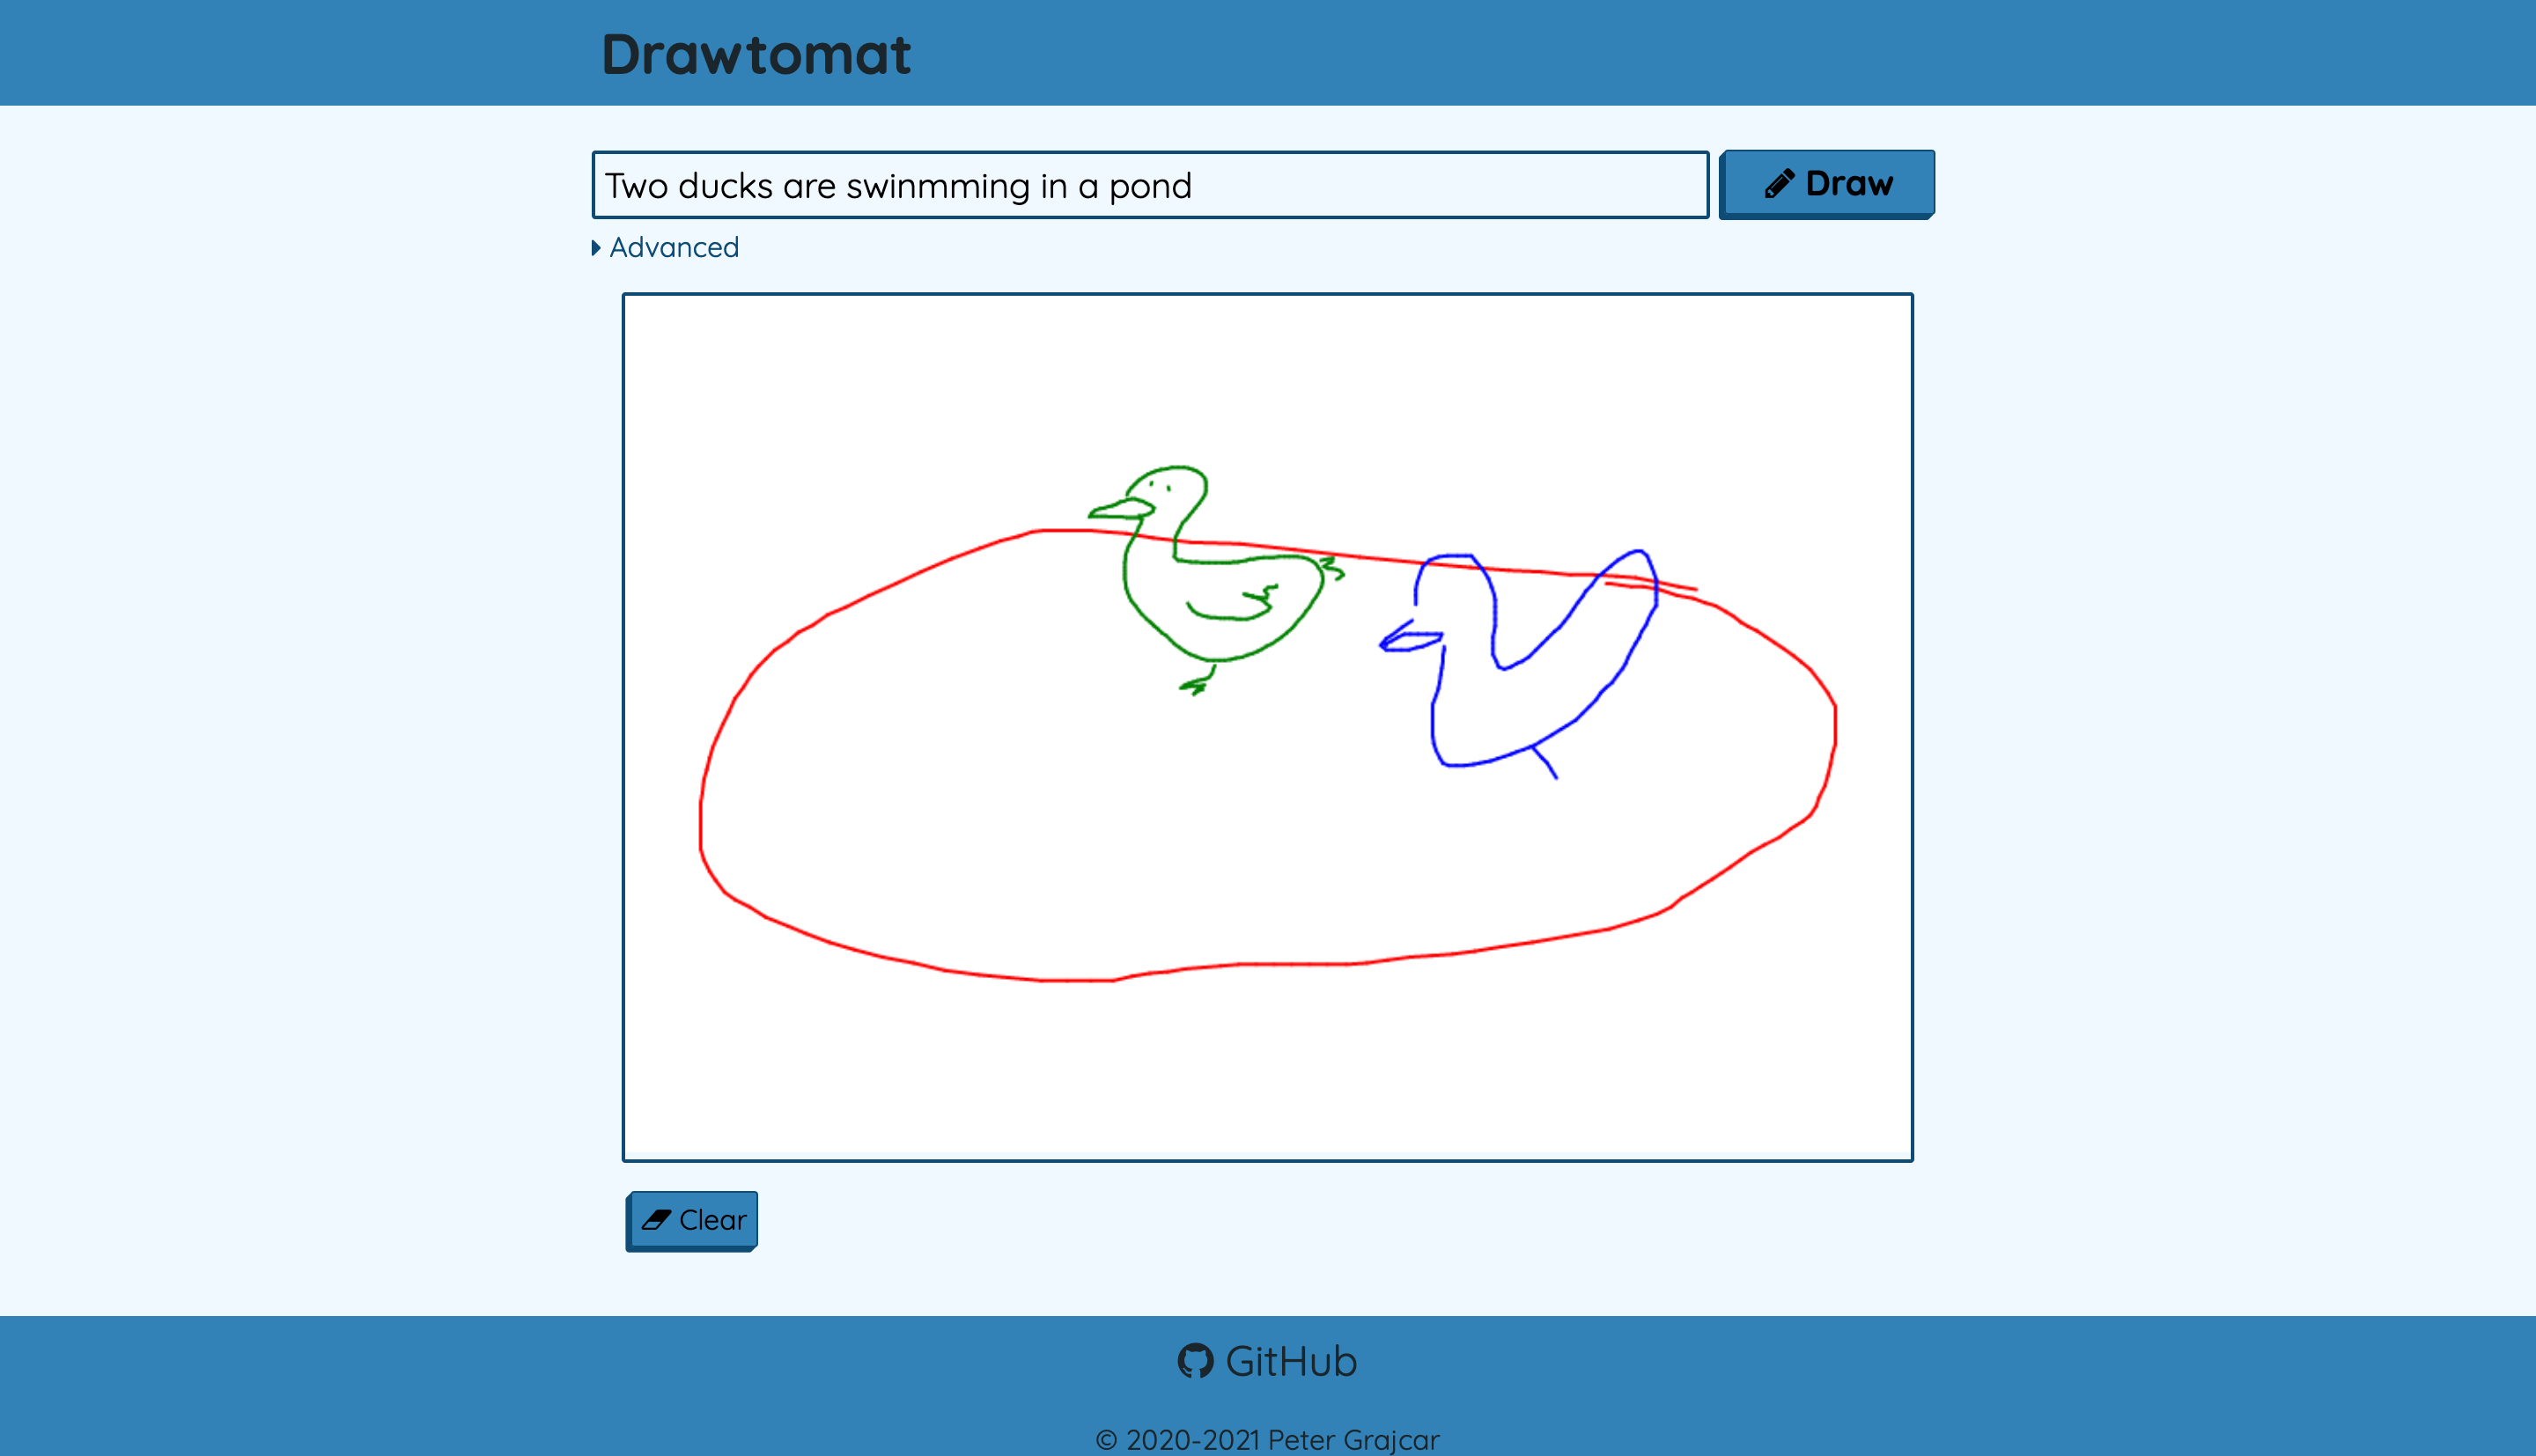
\includegraphics[width=\textwidth]{figures/web_client_1.png}
    \vskip 30pt
    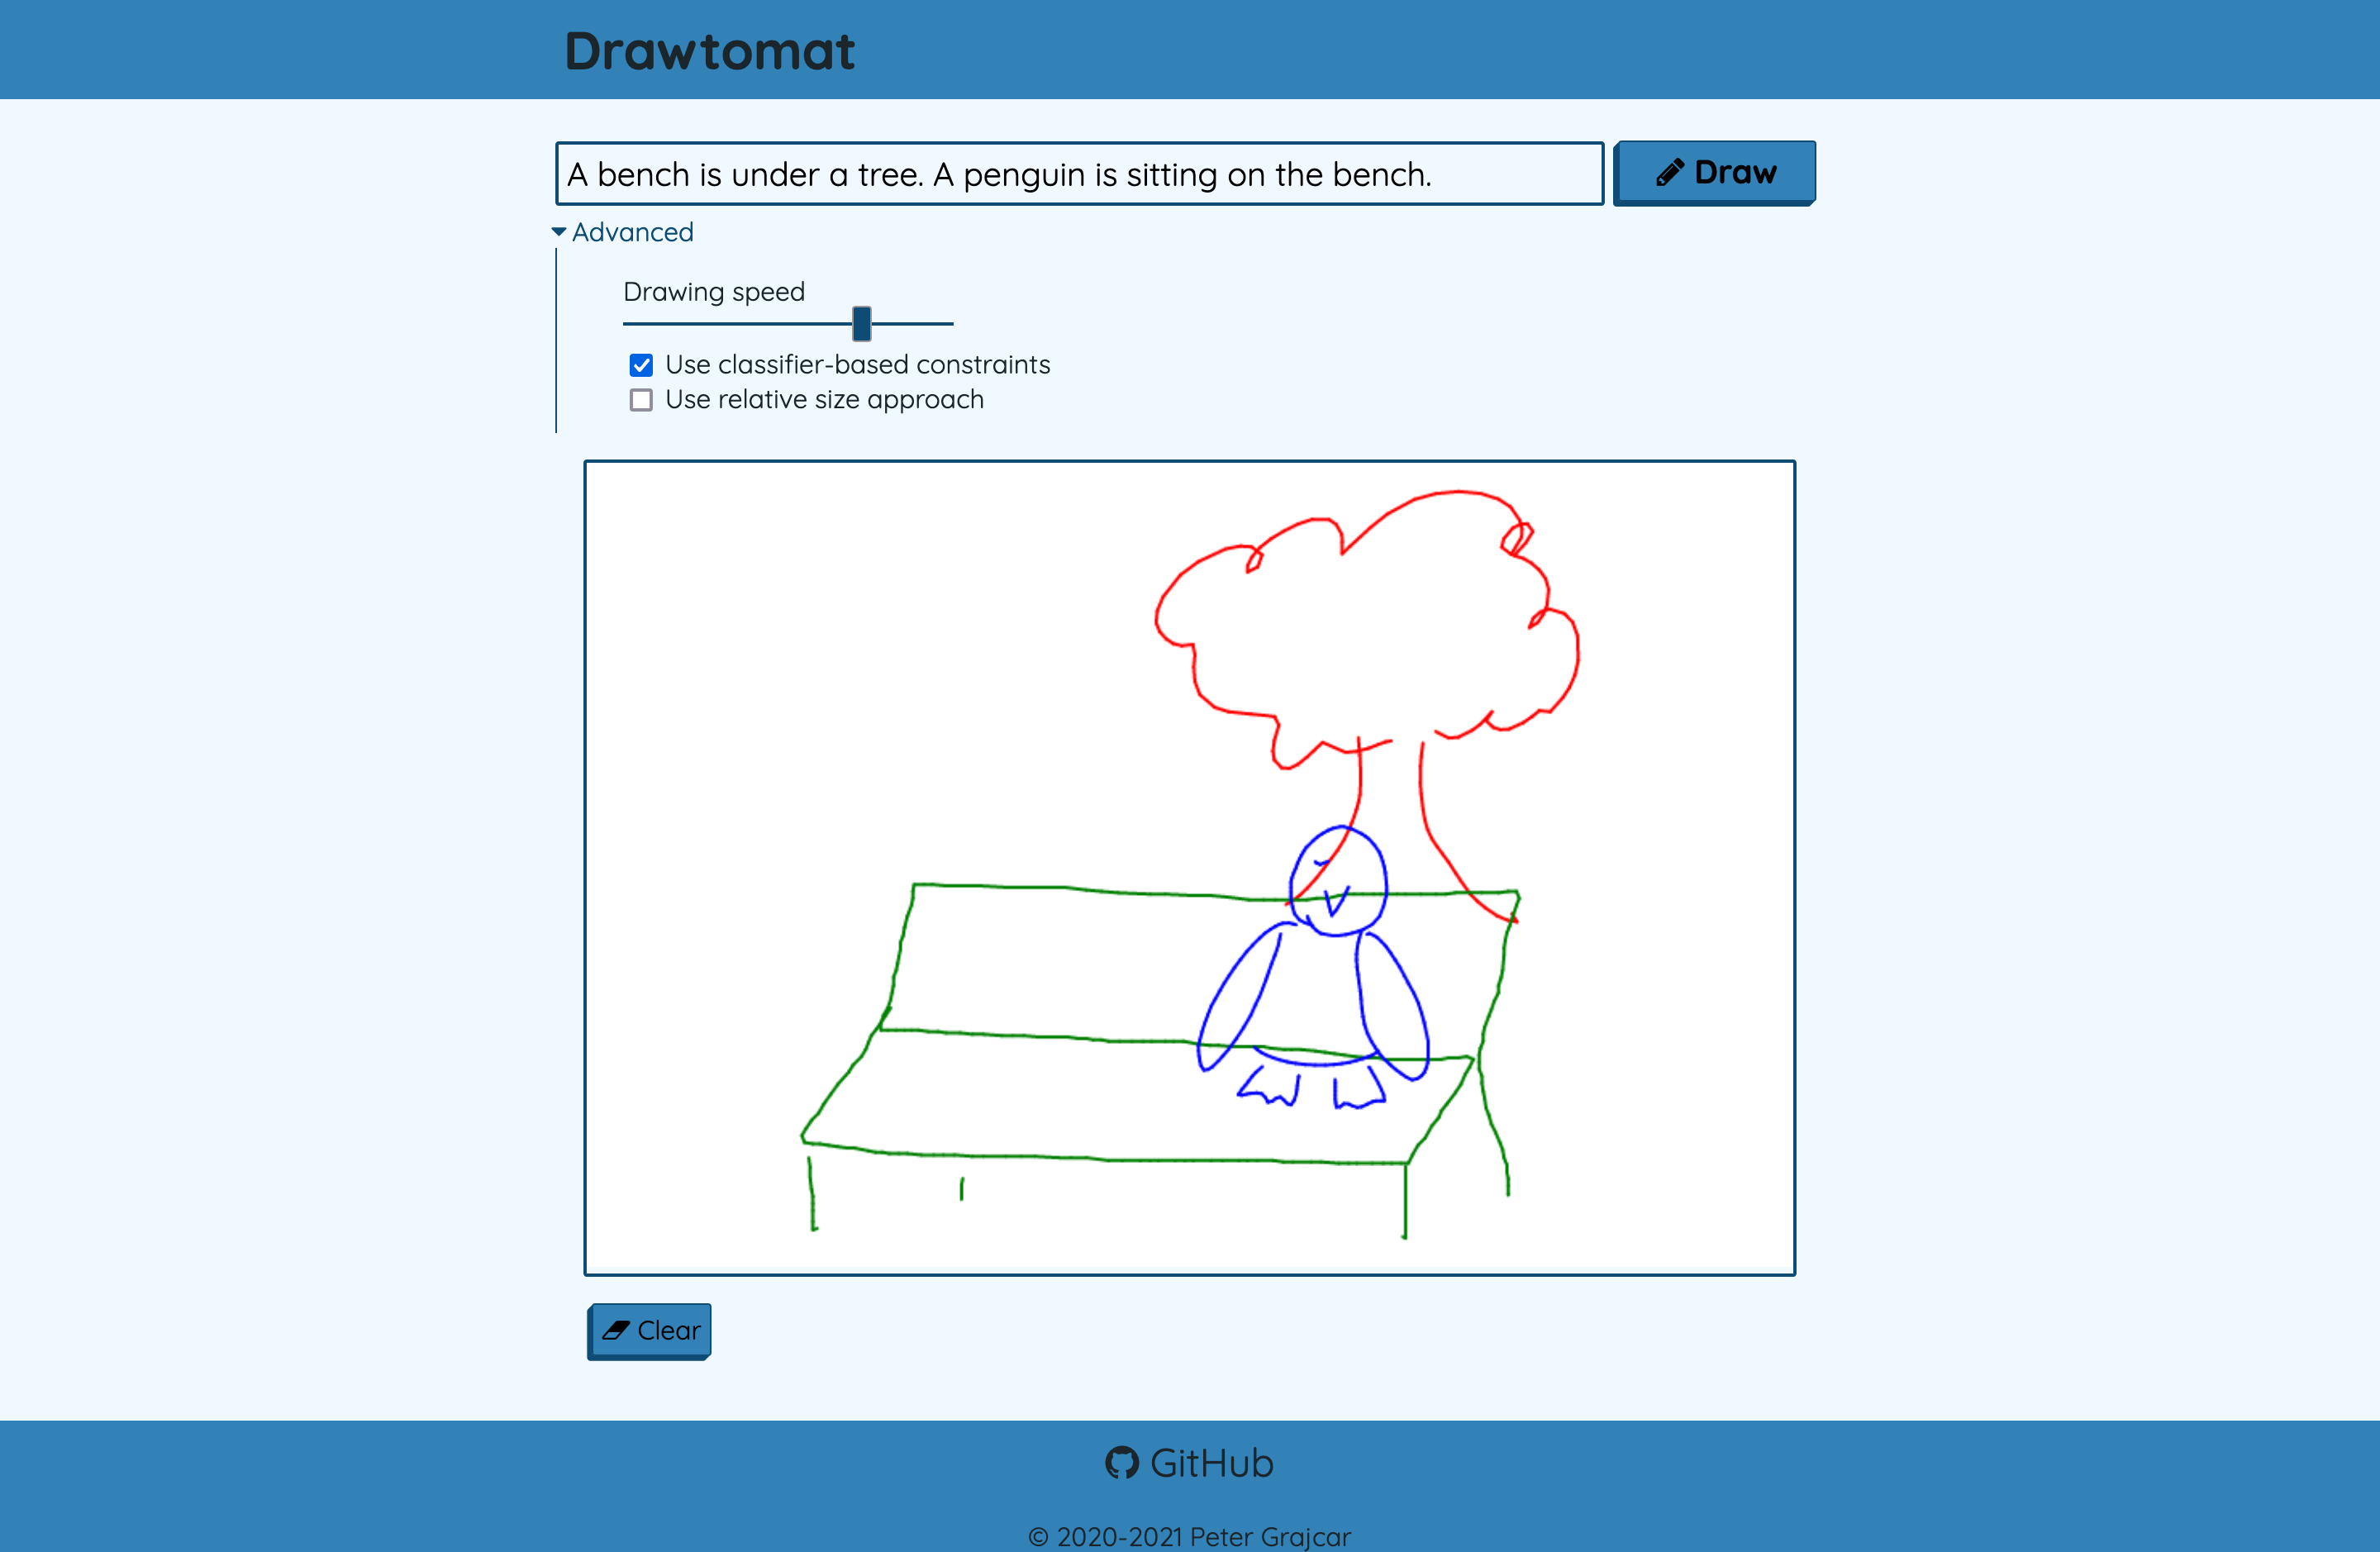
\includegraphics[width=\textwidth]{figures/web_client_2.png}
    \caption[The web client]{The web client.}
    \label{fig:web_client}
\end{figure}
